\documentclass[a4paper,10pt]{article}
\usepackage[utf8]{inputenc}

% ----  Useful packages % ---- 
\usepackage{amsmath}
\usepackage{graphicx}
\usepackage{amsfonts}
\usepackage{amsthm}
\usepackage{amssymb}
\usepackage{makecell}
% ----  Useful packages % ---- 

\usepackage{wrapfig}
\usepackage{caption}
\usepackage{subcaption}
\usepackage{hyperref}
\hypersetup{
	colorlinks,
	citecolor=black,
	filecolor=black,
	linkcolor=black,
	urlcolor=black
}

% ---- Set page size and margins replace ------
\usepackage[letterpaper,top=2cm,bottom=2cm,left=3cm,right=3cm,marginparwidth=1.75cm]{geometry}
% ---- Set page size and margins replace ------

% ------- NOTA ------
\theoremstyle{remark}
\newtheorem{note}{Note}[subsection]
% ------- NOTA ------

% ------- OSSERVAZIONE ------
\theoremstyle{definition}
\newtheorem{observation}{Osservazione}[subsection]
% ------- OSSERVAZIONE ------

% ------- DEFINIZIONE ------
\theoremstyle{plain}
\newtheorem{definition}{Definizione}[subsection]
% ------- DEFINIZIONE ------

% ------- ESEMPIO ------
\theoremstyle{definition}
\newtheorem{example}{Esempio}[subsection]
% ------- ESEMPIO ------

% ------- DIMOSTRAZIONE ------
\theoremstyle{definition}
\newtheorem{demostration}{Dimotrazione}[subsection]
% ------- DIMOSTRAZIONE ------

% ------- TEOREMA ------
\theoremstyle{definition}
\newtheorem{theorem}{Teorema}[subsection]
% ------- TEOREMA ------

% ------- COROLLARIO ------
\theoremstyle{plain}
\newtheorem{corollaries}{Corollario}[theorem]
% ------- COROLLARIO ------

% ------- PROPOSIZIONE ------
\theoremstyle{plain}
\newtheorem{proposition}{Proposizione}[subsection]
% ------- PROPOSIZIONE ------

% ---- Footer and header ---- 
\usepackage{fancyhdr}
\pagestyle{fancy}
\fancyhf{}
\fancyhead[LE,RO]{A.A 2023-2024}
\fancyhead[RE,LO]{Green Computing}
\fancyfoot[RE,LO]{\rightmark}
\fancyfoot[LE,RO]{\thepage}

\renewcommand{\headrulewidth}{.5pt}
\renewcommand{\footrulewidth}{.5pt}
% ---- Footer and header ---- 

% ----  Language setting ---- 
\usepackage[italian, english]{babel}
% ----  Language setting ---- 

\usepackage{listings}
\usepackage{color}

\definecolor{dkgreen}{rgb}{0,0.6,0}
\definecolor{gray}{rgb}{0.5,0.5,0.5}
\definecolor{mauve}{rgb}{0.58,0,0.82}

\lstset{frame=tb,
	language=C,
	aboveskip=3mm,
	belowskip=3mm,
	showstringspaces=false,
	columns=flexible,
	basicstyle={\small\ttfamily},
	numbers=none,
	numberstyle=\tiny\color{gray},
	keywordstyle=\color{blue},
	commentstyle=\color{dkgreen},
	stringstyle=\color{mauve},
	breaklines=true,
	breakatwhitespace=true,
	tabsize=3
}

\title{\textbf{Green Computing}}
\author{Realizzato da: Ghirardini Filippo}
\date{A.A. 2023-2024}

\begin{document}
	\begin{titlepage} %crea l'enviroment
	\begin{figure}[t] %inserisce le figure
		\centering
\includegraphics[width=0.98\textwidth]{marchio_unipi_pant541.png}
	\end{figure}
	\vspace{20mm}
	
	\begin{Large}
		\begin{center}
			\textbf{Dipartimento di Informatica\\ Corso di Laurea Triennale in Informatica\\}
			\vspace{20mm}
			{\LARGE{Corso a Libera Scelta - 6 CFU}}\\
			\vspace{10mm}
			{\huge{\bf Computer Graphics}}\\
		\end{center}
	\end{Large}
	
	
	\vspace{36mm}
	%minipage divide la pagina in due sezioni settabili
	\begin{minipage}[t]{0.47\textwidth}
		{\large{\bf Professore:}\\ \large{Prof. }}
	\end{minipage}
	\hfill
	\begin{minipage}[t]{0.47\textwidth}\raggedleft
		{\large{\bf Autore:}\\ \large{Filippo Ghirardini}}
	\end{minipage}
	
	\vspace{25mm}
	
	\hrulefill
	
	\vspace{5mm}
	
	\centering{\large{\bf Anno Accademico 2023/2024 }}
	
\end{titlepage}
	
	\tableofcontents
	\newpage
	\maketitle
	\begin{center}
		\vspace{-20pt}
		\rule{11cm}{.1pt} 
	\end{center}
	\section{Punto materiale}
Oggetto caratterizzato da una massa [kg] e da un vettore posizione [m] nello spazio 3D.
Dimensioni trascurabili, forma irrilevante rispetto ai fenomeni di interesse.
Vettore posizione come funzione del tempo t[s].
\begin{example}
    Una molecola di ossigeno se sono interessato all'aereodinamica di una vettua. 
    Un satellite attorno alla terra se ignoro le forze di marea.
\end{example}
\hspace{-15pt}\textbf{Un vettore posizione} è una funzione del tempo $t[s]$.
$$\vec{r(t)} = (x(t), y(t), z(t)) = x(t)\hat{x} + y(t)\hat{z} + z(t)\hat{z}$$
\begin{observation}
    I versori cartesiani sono costanti
\end{observation}

\begin{definition}[Legge oraria]
    Si definisce come legge oraria la funzione $t \mapsto \vec{r}(t)$.
\end{definition}

\begin{definition}[Traiettoria]
    Il luogo geometrico di punti visitati dal punto materiale.
    $$\{\vec{r}(t)\:\: per \: t \in \mathbb{R}\}$$
\end{definition}

\begin{example}
    $\vec{r}(t) = (v_0t, y_0, 0)$ e $v_0 = 3m/s, y_o = 5m$ 
    \begin{figure}[h!]
        \centering
        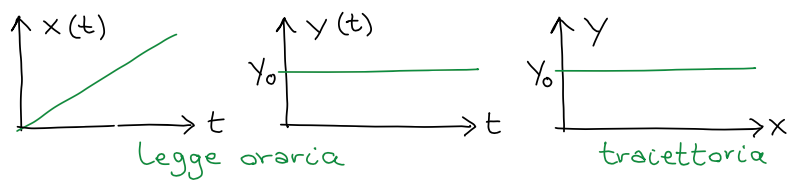
\includegraphics[width=0.8\textwidth]{images/ess-traiettoria.png}
    \end{figure}
\end{example}

\begin{definition}
    La \textbf{velocità istantanea} è la derivata della posizione rispetto al tempo.
    $$v = \lim_{\Delta t \to 0}\frac{\Delta s}{\Delta t} = \frac{ds}{dt}$$
\end{definition}

\begin{definition}
    La \textbf{velocità media} è definita come il rapporto tra lo spostamento e l'intervallo di tempo necessario per effettuarlo.
    $$v_m = \frac{\Delta s}{\Delta t}$$
\end{definition}
\hspace{-15pt}In parole povere è una grandezza che ci dice con quale rapidità cambia la posizione di un punto rispetto al tempo nell'instante $t$.
\subsection*{Vettore velocità}
Derivata rispetto al tempo del vettore posizione e si indica come 
$\frac{d\vec{r}(t)}{dt}\text{ oppure }\dot{\vec{r}}(t)[m/s]$
\begin{equation}
    \begin{split}
    \dot{\vec{r}}(t) & = (\dot{x}(t), \dot{y}(t), \dot{z}(t)) \\
     & = \frac{d}{dt}[x(t)\hat{x} + y(t)\hat{y} + z(t)\hat{z}] \\
     & = \dot{x}(t)\hat{x} + \dot{y}(t)\hat{y} + \dot{z}(t)\hat{z}
    \end{split}
\end{equation}
Per ricavare la forma esplicita uso le proprietà delle derivate (\textbf{linearità}, \textbf{Leibnitz})
\begin{example}
    $\vec{r}(t) = (v_0t, y_0, 0) = v_0t\hat{x} + y_0\hat{y}$ \:\:\:abbiamo che \:\:\:
    $\dot{\vec{r}}(t) = (v_0, 0, 0) = v_0 \hat{x}$
\end{example}
\hspace{-15pt}Velocità e spazio percorso ("integrale di linea").\\
\begin{wrapfigure}[3]{l}{5cm}
    \centering
    \includegraphics[width=5cm]{images/vettore-velocità.png}
\end{wrapfigure}
\begin{align*}
    L & = ||\vec{r}(t_1) - \vec{r}(t_0)|| + ||\vec{r}(t_2) - \vec{r}(t_1)|| + ||\vec{r}(t_3) - \vec{r}(t_2)|| + \dots \\
    & = \sum_i ||\vec{r}(t_{i+1} - \vec{r}(t_i)|| \:\: per\:\: |t_{i+1} - t_i| \text{"piccolo"} \\
    & = \sum_i ||\frac{\vec{r}(t_{i+1}) - \vec{r}(t_i)}{t_{i+1} - t_i}|| (t_{i+1} - t_i) = \int_{t_{in}}^{t_{f_{in}}}||\dot{\vec{r}}(t)||\\
\end{align*}
\begin{example}
    $\vec{r}(t) = (v_0t, y_0)\:\:\: \dot{\vec{r}}(t) = (v_0, 0)$\hspace{15pt}
    $||\dot{\vec{r}}(t)|| = \sqrt{v_0^2 + 0^2} = |v_0|$ \:\:\: $L = |v_0| \cdot (t_{f_{in}} - t_{in})$\\
    Il vettore è costante quindi facendo la derivata torna zero. Con la velocità si calcolo lo spazio percorso ("integrale di linea").
    La differenza fra le posizioni e la differenza dei tempi è il rapporto incrementale in caso gli intervalli siano sufficentemente
    piccoli, da qui si ottiene l'integrale.
\end{example}

\subsection{Vettore accelerazione}
Derivata rispetto al tempo del vettore velocità e si indica con $\frac{d^2\vec{r}(t)}{dt} \text{ oppure } \ddot{\vec{r}}(t) [m/s^2]$
\begin{equation}
    \ddot{\vec{r}}(t) = (\ddot{x}(t), \ddot{y}(t), \ddot{z}(t))\:\: = \:\: \ddot{x}(t)\hat{x} + \ddot{y}(t)\hat{y} + \ddot{z}(t)\hat{z}
\end{equation}
\begin{example}
    $\vec{r}(t)= (\frac{1}{2}a_0t^2, v_0t, 0)$ \hspace{10pt} $\dot{\vec{r}}(t) = (a_0t, v_0, 0)$ \hspace{10pt} $\dot{\vec{r}}(t) = (a_0, 0, 0)$
\end{example}
\hspace{-15pt}Serve perché l'equazione "del moto" di Newton che determinata la legge oraria è formulata in termini di accelerazione.

\subsection{Vettore quantità di moto}
Il prodotto di massa [kg] e velocità [m/s]
$$\vec{p}(t) = m \cdot \dot{\vec{r}}(t) = (m\dot{x}(t), m\dot{y}(t), m\dot{x}(t)) = m\dot{\vec{x}}(t)x + m\dot{\vec{y}}(t)y + m \dot{\vec{z}}(t)z$$
\begin{example}
    Prendiamo un punto di massa 2kg e velocità 3m/s lungo $\hat{x}$.\\
    $p_x(t) = 2 \cdot 3 kg\cdot m/s = 6 kg \cdot m/s$ \hspace{15pt} $p_y(t) = p_z(t) = 0$.
\end{example}
\hspace{-15pt}Serve per generalizzare l'equazione di Newton e per trattare sistemi di piu punti materiali.

\subsection{Vettore momento angolare rispetto a un polo P}
$$\vec{L}_p(t) = m(\vec{r}(t) - \vec{r}_p) \times \dot{\vec{r}}(t)$$
Dove $\vec{r}_p$ è il vettore posizione di p, mentre $\dot{\vec{r}}(t)$ è il prodotto vettoriale.
\begin{example}
    $\vec{r}_p = (l_0, 0, 0)$ \hspace{15pt} $\vec{r}(t) = (v_0t, y_0, 0)$\\
    $\vec{L}_p = m[(v_0t - l_0)\hat{x} + y_0\hat{y}] \times (v_0\hat{x}) \:\: = \:\: m(v_0t - l_0)v_0 \hat{x} \times \hat{x} + my_0v_0\hat{y}\times \hat{x} 
    \:\: = \:\: my_0v_0(-\hat{z}) = (0,0, -my_0v_0)$\\
    Ricorda che $\hat{x} \times \hat{x} = 0$ e $\hat{y} \times \hat{x} = -\hat{z}$
\end{example}
\hspace{-15pt}Il momento angolare dice quanta inerzia ha un oggetto in una rotazione (descrizione sommaria).\\
Il polo P è parte della definizione. È una scelta! Il risultato dipende dal polo.
Serve per formulare l'equazione del moto di sistemi di punti materiali e corpi rigidi.

\subsection{Coordinate polari}
Un metodo per rapprensentare delle cordinate x, y andando a misurare prima la distanza dall'origine e poi si va a vedere
quanto vale l'angolo fra questo segmento dall'asse x, utilizzando seno e coseno.
\begin{wrapfigure}[7]{l}{2cm}
    \centering
    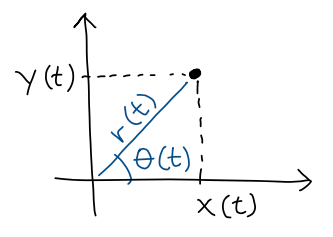
\includegraphics[width=5.5cm]{images/coordinate-polari.png}
\end{wrapfigure}
\begin{align*}
    \begin{cases}
        x(t) = r(t) \cdot \cos(\Theta(t))\\
        y(t) = r(t) \cdot \sin(\Theta(t)) 
    \end{cases}
\end{align*}
\begin{align*}
    \begin{cases}
        r(t) = \sqrt{x(t)^2 + y(t)^2} \geq 0\\
        tg(\Theta(t)) = y(t) / x(t) 
    \end{cases}
\end{align*}
\\
\begin{example} Esempi di rappresentazione di coordinate in coordinate polari.\\
    $x = 0, y = l_0 > 0 \:\: \Rightarrow \:\: r = l_0, \Theta = \pi/2$\\
    $x = 0, y = -l_0 < 0 \:\: \Rightarrow \:\: r = l_0, \Theta = -\pi/2$\\
    $x = l_0, y = l_0 > 0 \:\: \Rightarrow \:\: r = \sqrt{2}l_0, \Theta = \pi/4$\\
\end{example}

\subsection{Versori polari (2D)}
Definisco un versore $\hat{r}(t)$ che punta verso il punto materiale e un versore $\hat{\Theta}(t)$ ortogonale.
Si esprime facilmente in coordinte polari.
$$\vec{r}(t) = (x(t), y(t)) = (r(t)\cos \Theta(t), r(t)\sin\Theta(t)) \:\: = \:\: r(t)(\cos\Theta(t)\hat{x} + \sin\Theta(t)\hat{y})$$
Ma $||\vec{r}(t)|| = |r(t)| = r(t)$ allora definisco $\hat{r}(t) = \vec{r}(t)/ ||\vec{r}(t)|| = \cos \Theta(t)\hat{x} + \sin\Theta(t)\hat{y}$\\\\
Trovo facilmente che un versore ortogonale è:
$$\hat{\Theta(t)} = -\sin\Theta(t)\hat{x} + \cos\Theta(t)\hat{y} \:\:\:\text{infatti} \:\:\: \hat{r}\cdot \hat{\Theta} = c \cdot (-s) + s \cdot c = 0$$
\begin{wrapfigure}[7]{r}{6cm}
    \centering
    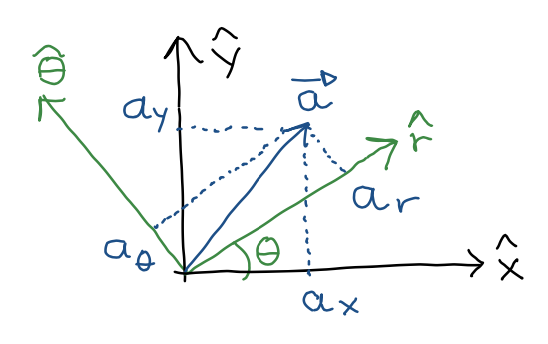
\includegraphics[width=5.5cm]{images/trasformazioni-inverse.png}
\end{wrapfigure}
\begin{note}
    Non c'è legame fra $\Theta$ e $\hat{\Theta}$ è solo una convenzione.
\end{note}
\hspace{-15pt}Le trasformazioni inverse invece si fanno come segue (verifico per sostituzione):
$$\hat{y} = \cos\Theta(t)\hat{r} - \sin\Theta(t)\hat{\Theta} \hspace{20pt} \hat{y} = \sin\Theta(t)\hat{r} + \cos\Theta(t)\hat{\Theta}$$
Possono quindi scrivere ogni vettore nella forma $\vec{a} = a_r\hat{r} + a_{\Theta}\hat{\Theta}$ con le componenti polari $a_r, a_{\Theta}$.
Per evitare ambiguità non scriviamo $(a_r, a_{\Theta})$ e riserviamo la notazione alle componenti cartesiane.\\\\
A differenza dei versori cartesiani quelli polari dipendono dal tempo per costruzioni.
$$\dot{\hat{r}}(t) = \frac{d}{dt}[\cos\Theta(t) \hat{x} + \sin\Theta(t)\hat{y}] \:\: = \:\: -\sin\Theta(t) \cdot \dot{\Theta}(t)\hat{x} + \cos\Theta(t) \cdot \dot{\Theta}(t)\hat{y}$$
Dove $\cos\Theta(t) \cdot \dot{\Theta}(t)$ si applica la derivata della somma, Leibnitz, funzione composta.
$$= \dot{\Theta}(t)\cdot \hat{\Theta}(t) \:\:\:\:(\text{confronto l'espressione di} \hat{\Theta}(t))$$
Similmente $\dot{\hat{\Theta}}(t)= - \dot{\Theta}\hat{r}(t)$.


\subsection*{Vettori posizione, velocità, accelerazione}
$$\vec{r}(t) = r(t)\hat{r}(t)$$
Dove abbiamo che $\vec{r}(t)$ è il vettore, $r(t)$ è una coordinata polare, $\hat{t}(t)$ è il versore polare.
$$\dot{\vec{r}}(r) = \dot{r}(t)\hat{r}(t) + r(t)\dot{\Theta}(t)\hat{\Theta}(t)$$
Dove la parte $\dot{\vec{r}}(r)$ è la velocità radiale.
$$\ddot{\vec{r}}(t) = [\ddot{r}(t) - r(t)\dot{\Theta}(t)^2] \hat{r} + [r(t) \ddot{\Theta}(t) + 2\dot{r}(t)\dot{\Theta}(t)]\hat{\Theta}$$
Nel quale abbiamo che la parte $r(t)\dot{\Theta}(t)^2$ si chiama \textbf{velocità centripeta}, mentre $2\dot{r}(t)\dot{\Theta}(t)$ si dice \textbf{accelerazione di Coriolis}.


	% !TeX spellcheck = it_IT
\newpage
\section{Green Computing}
In generale, il green computing può aiutare le organizzazioni a ridurre l'impatto ambientale e a risparmiare sui costi energetici e di gestione.

\begin{definition}[Green Computing]
	Il green computing tratta la \textbf{progettazione}, la \textbf{realizzazione} e l'\textbf{utilizzo} di \underline{sistemi ICT}, \underline{computer} e \underline{dispositivi elettronici}\footnote{Tutti quei dispositivi che si appoggiano all'informatica per funzionare, e.g. aspirapolvere} in modo responsabile e sostenibile dal punto di vista ambientale, considerando in particolare il \textbf{consumo energetico} e \textbf{impronta di carbonio}.
\end{definition}

\begin{definition}[$CO_2$-eq]
	L'anidride carbonica equivalente è una misura che esprime l'impatto di una certa quantità di gas serra rispetto alla stessa quantità di anidride carbonica.
\end{definition}

\begin{definition}{Energy Star}
	Il progetto Energy Star nasce negli anni '90 ed è stata una delle prime iniziative relative al green computing per dare un indicatore dell'efficienza energetica. Il problema principale è che è \textbf{facoltativo}.
\end{definition}

\subsection{Approccio olistico}
Per funzionare segue un approccio \textbf{olistico}, analizzando tutto il \textbf{ciclo di vita} di un sistema, sia \emph{vericalmente} che \emph{orizzontalmente}.

\begin{itemize}
	\item \textbf{Progetto}: progettare in modo sostenibile computer, server, sistemi di raffreddamento e software a basso consumo e alta efficienza.
	\item \textbf{Produzione}: attenzione a non sprecare risorse limitate, ridurre gli scarti di fabbricazione e utilizzare fonti rinnovabili per la produzione.
	\item \textbf{Trasporto}: cercare di ridurre e ammortizzare l'uso di carburanti fossili sostituendoli con veicoli elettrici o ibridi e facendo spedizioni accorpate.
	\item \textbf{Uso}: utilizzare i sistemi cercando di ridurre il consumo con politiche di risparmio (e.g. ibernazione)
	\item \textbf{Dismissione}: lo smaltimento di dispositivi elettronici attraverso il riciclo
\end{itemize}

\subsection{Pilastri fondamentali}
\begin{center}
	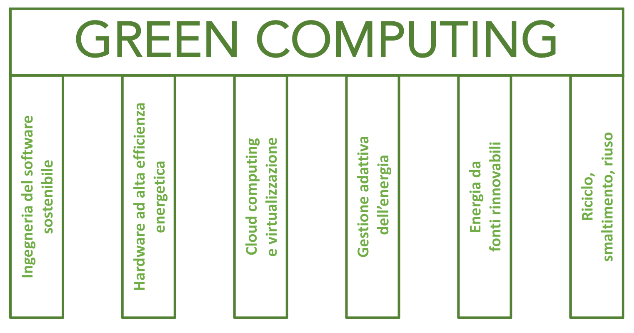
\includegraphics[scale=0.5]{green_pilastri.png}
\end{center}
\subsubsection{Ingegneria del software sostenibile}
È possibile fare in modo che i programmi consumino meno energia e che il loro dispiegamento nelle varie fasi del ciclo di vita produca minori gas inquinanti. In particolare, programmare \emph{sfruttando le peculiarità di linguaggi e hardware} che possano rendere il software più disponibile.
\subsubsection{Hardware ad alta efficienza energetica}
L'hardware ad alta \textbf{efficienza energetica} o le configurazioni Eco permettono di ridurre l'impatto ambientale e risparmiare sui costi energetici e di gestione. Inoltre, sistemi di raffreddamento più efficienti e processori di nuova generazione consumano meno. Alcune \textbf{periferiche} a basso consumo energetico sono:
\begin{itemize}
	\item Schermi OLED:  I pixel dello schermo si spengono su immagini nere risparmiando energia
	\item Stampanti, scanner, etc.
\end{itemize}
Va considerato un trade-off tra prestazioni e consumi, con l'obiettivo di avere un minore impatto ambientale
\subsubsection{Cloud computing e virtualizzazione}
Il Cloud Computing permette di \textbf{condividere} le risorse informatiche tra più utenti e organizzazioni, riducendo così gli sprechi di risorse. Inoltre, le grandi aziende che forniscono servizi cloud possono permettersi di investire in infrastrutture tecnologiche più \textbf{efficienti} dal punto di vista energetico, per esempio utilizzando fonti rinnovabili per alimentare i propri data center. Inoltre, il cloud computing permette una maggiore \textbf{flessibilità} nell'allocazione delle risorse, garantendo l'accesso (anche elastico) solo alle risorse necessarie per un'applicazione specifica. Ciò si traduce in una riduzione del consumo energetico. La virtualizzazione delle risorse consente di \textbf{ottimizzare} l'utilizzo hardware, riducendo così gli sprechi.
\subsubsection{Gestione adattiva dell'energia}
La gestione adattiva dell'energia permette di abbattere i consumi e i costi tramite metodi su più livelli, appiattendo la curva di consumo energetico, risparmiando soldi e risorse e riducendol’utilizzo di energia nelle ore di basso utilizzo. Alcuni esempi sono:
\begin{itemize}
	\item \textbf{Adattività del raffreddamento}: ridurre/aumentare il raffreddamento in base all’utilizzo del processore, può portare fino ad una riduzione del 20\% dei consumi
	\item \textbf{Batteria}: aumento della vita della batteria evitando di stressarla utilizzando l’energia della presa quando in carica
	\item \textbf{Sistemi operativi}: Adaptive job scheduling e timing di spegnimento e sospensione dello schermo e del sistema
	\item \textbf{Illuminazione adattiva dei dispositivi mobil}i: la maggior parte dei nuovi dispositivi sono in grado di adattare la luminosità del display in base alla luminosità ambientale
\end{itemize}
\subsubsection{Energia da fonti rinnovabili}
La transizione verde ha come pilastro fondamentale il passaggio da un sistema basato per la quasi totalità su fonti energetiche inquinanti a un modello virtuoso incentrato invece su fonti rinnovabili. Utilizzare \textbf{fonti rinnovabili} per alimentare i data center e i dispositivi informatici può quindi ridurre significativamente le emissioni di CO2 e 
contribuire a combattere il cambiamento climatico.
\subsubsection{Riciclo, smaltimento, riuso}
È possibile \textbf{sensibilizzare} l'utente sul giusto uso dei mezzi a sua disposizione e quindi della loro conseguente fine di utilizzo. Ottimizzare l'impiego dei dispositivi porta una determinante longevità, minimizzando quindi il rifiuto.
\begin{itemize}
	\item Inoltre, per ridurre la produzione di rifiuti è fondamentale \textbf{riutilizzare} (ad esempio rivendendo) i dispositivi elettronici ancora validi. In molti casi è sufficiente sostituire componenti degradati (e.g. le batterie) e mantenere il resto. Oltretutto molti dispositivi possono essere considerati obsoleti per certi scopi ma ancora ottimi per altri (e.g. server).
	\item È fondamentale ingegnerizzare il processo di \textbf{smaltimento} in modo da permettere il \textbf{riciclo} di parte dei componenti. Ad esempio dalle schede stampate si possono recuperare metalli preziosi come l'oro. La legislazione italiana necessita il corretto trattamento dei rifiuti per ridurre l'inquinamento. Di conseguenza anche la scelta di macchinari e strumenti mirati allo smaltimento è fondamentale per fare in modo che un'azienda possa essere ritenuta green.
	\item La tecnologia stessa può essere uno strumento potente per \textbf{sensibilizzare} il consumatore su queste tematiche e per fargli conoscere le aziende green.
\end{itemize}
\subsection{Applicazioni green}
Sfruttare i sistemi ICT per l'\textbf{ottimizzazione} di processi che sfruttano risorse limitate (e.g. combustibili fossili nel trasporto, energia elettrica nel riscaldamento, acqua potabile nell'irrigazione) è un aspetto importante del green computing.
\end{document}
